\chapter{高水準入出力と低水準入出力}

ファイルを読み書きするための機能(API:Application Program Interface)は,
C言語の入門で勉強した高水準入出力と,
前の章で勉強した低水準入出力(システムコール)の2種類がある.
この章では高水準入出力と低水準入出力の関係を学ぶ.
なお,以下では高水準入出力のことを{\em 高水準I/O},
低水準入出力のことを{\em 低水準I/O}と呼ぶことがある.

高水準I/O関数は,様々な機能を持つものが豊富に用意されており,
プログラマーが便利に使用することができる.
一方で OS カーネルの出入り口であるシステムコールの種類は少なくし,
メモリに常駐する OS カーネルをシンプルにしている.

%----------------------------------------------------------------------
\section{高水準I/Oのデータ構造}
高水準I/O関数は\|fopen()|が返したファイルポインタを用いて入出力先を区別する.
以下ではファイルポインタが指すデータ構造について説明する.

\subsection{FILE構造体}
高水準I/Oと低水準I/Oの関係を\figref{HiVsLoWrite}に示す.
図で \|fp| は FILE 型のポインタ({\em ファイルポインタ})である.
\|fp|は,\|fopen()| が作成し初期化したFILE 構造体を指している.
FILE 構造体の内部には,
管理データ,データのバッファ,ファイルディスクリプタ(\|fd|)等が格納される.
\|fd|の値は,
\|fopen()|が open システムコールを実行した時に決められる.

\begin{myfig}{btp}{高水準と低水準の関係(書き込みの場合)}{HiVsLoWrite}
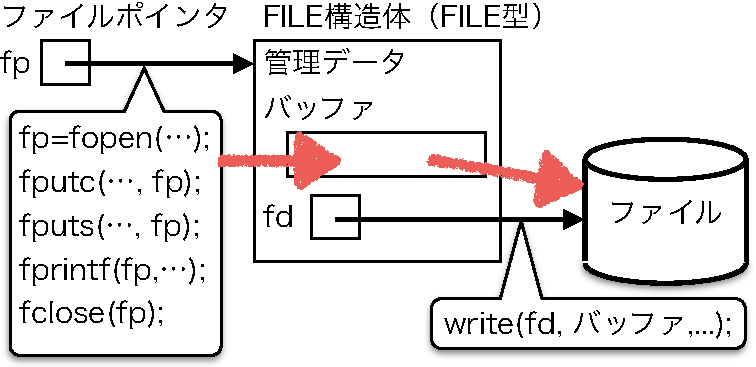
\includegraphics[scale=0.7]{Fig/HiVsLoWrite-crop.pdf}
\end{myfig}

\subsection{バッファの役割}
\figref{HiVsLoWrite}に示したように,
高水準I/O関数は出力データを FILE 構造体の内部にある{\em バッファ}に書き込む.
データはバッファがいっぱいになった時,
または,その他,一定の条件を満たした時に
\texttt{write()} システムコールによってファイルに書き込まれる.
これは FILE 構造体のバッファにデータをためることにより、
\texttt{write()} システムコールの実行回数を少なくする工夫である.
一般に{\em システムコールは重い処理}なので,
システムコールの実行回数が少なくなるような工夫が必要とされる
\footnote{\texttt{read()},\texttt{write()}システムコールの重さは,
一度に扱うデータの量にあまり左右されない.回数が重要である.}.

\figref{HiVsLoRead}に入力の場合を示す.
入力でもシステムコールの回数が少なくなるようにバッファを使用する.
入力の場合は\texttt{read()} システムコールでデータをバッファーにまとめて読み,
\|fgetc()| 等がバッファから入力データを必要に応じて取り出す仕組みになっている.

\begin{myfig}{btp}{高水準と低水準の関係(読み込みの場合)}{HiVsLoRead}
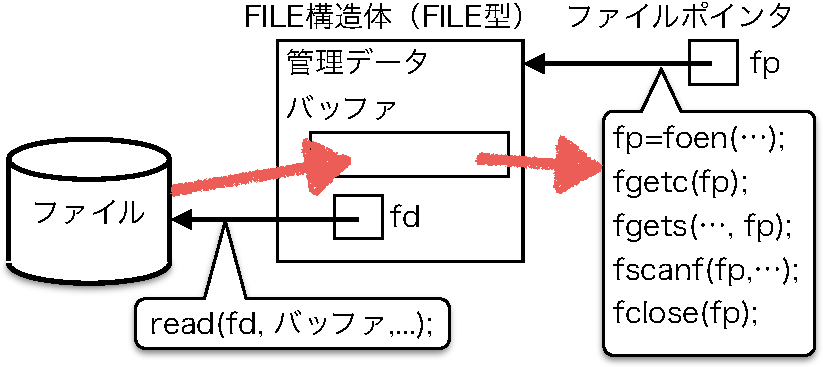
\includegraphics[scale=0.7]{Fig/HiVsLoRead-crop.pdf}
\end{myfig}

\section{標準入出力}
\|scanf()|,\|getchar()|,\|printf()|,\|putchar()|等は
引数にファイルポインタを持たない高水準I/O関数である.
プログラム実行開始時にオープンされたファイルポインタ\|stdin|や\|stdout|を,
これらは暗黙の内に使用する.
これらのファイルポインタを通して読み書きするデータの流れを
{\em 標準入出力ストリーム}と呼ぶ.
標準入出力ストリームの一覧と模式図を\tabref{stdio}と\figref{stdio}に示す.

\begin{mytable}{btp}{標準入出力ストリーム一覧}{stdio}
  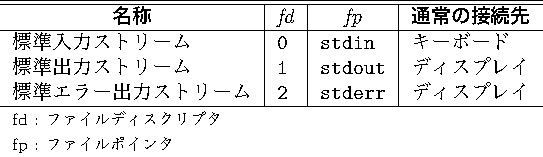
\includegraphics[scale=1.0]{Tbl/stdio.pdf}
\end{mytable}

\begin{myfig}{btp}{標準ストリームの構造}{stdio}
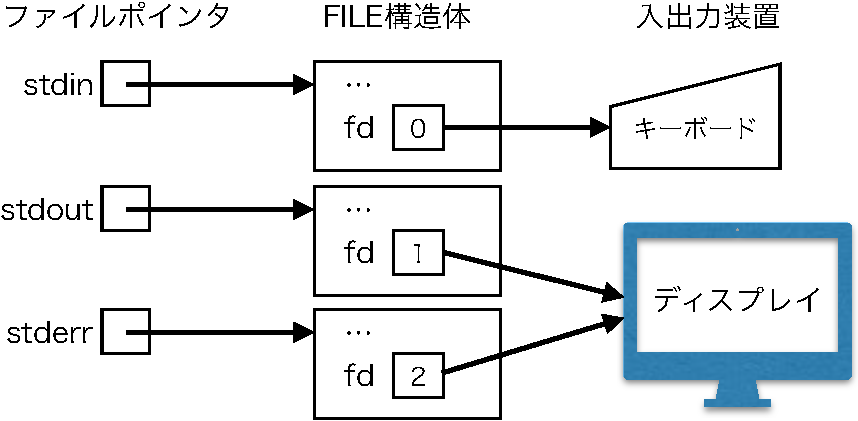
\includegraphics[scale=0.7]{Fig/stdio-crop.pdf}
\end{myfig}

\subsection{ユニファイドI/O}
標準入出力ストリームを使用する
\|scanf()|,\|getchar()|,\|printf()|,\|putchar()|等は,
ファイルポインタを引数に持つ
\|fscanf()|,\|fgetc()|,\|fprintf()|,\|fputc()|関数に
標準入出力ストリーム(\|stdin|,\|stdout|等)を渡した場合と同じ働きをする.
\tabref{printfVsFprintf}に同じ働きをする関数の対応を示す.
例えば\|getchar()|関数\footnote{正確には\texttt{getchar()}マクロ.}は,
\|fgetc()|の引数に標準入力ストリームを表す\|stdin|を
渡したものと同じ働きをする.

このようにファイルへの読み書きも,
キーボードやディスプレイ等の装置への入出力も,
ファイルポインタやファイルディスクリプタを用いて
同じ入出力関数や同じシステムコール(read/write)で行うことができる.
ファイルも装置も同様に(同じAPIで)扱う方式を{\em ユニファイドI/O}と呼ぶ.

\begin{mytable}{btp}{同じ役割をする入出力関数}{printfVsFprintf}
  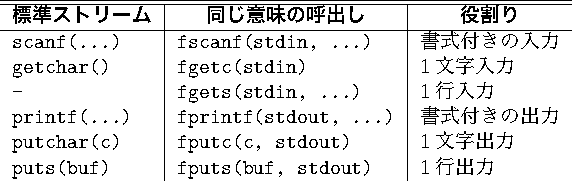
\includegraphics[scale=1.0]{Tbl/printfVsFprintf.pdf}
\end{mytable}

\subsection{標準入力ストリーム}
ファイルポインタ\|stdin|により参照され,
\|scanf()|や\|getchar()|等が暗黙に使用する入力ストリームである.
ファイルディスクリプタ 0 はプログラム起動前にオープンされている.
プログラムは起動時に\|FILE|構造体を作成し\figref{stdio}のように初期化する.

通常ファイルディスクリプタ 0 はキーホード用にオープンされるが,
ファイルにリダイレクトすることも可能である\footnote{
シェルで \texttt{<} を用いて
標準入力ストリームをファイルにリダイレクトすることができる.}.
リダイレクトはプログラムが起動される前にシェルによって行われる.

\subsection{標準出力ストリーム}
ファイルポインタ\|stdout|により参照され,
\|printf()|や\|putchar()|等が暗黙に使用する出力ストリームである.
ファイルディスクリプタ 1 はプログラム起動前にオープンされている.
プログラムは起動時に\|FILE|構造体を作成し\figref{stdio}のように初期化する.

通常ファイルディスクリプタ 1 はディスプレイ用にオープンされるが,
ファイルにリダイレクトすることも可能である\footnote{
シェルで \texttt{>} を用いて標準出力ストリームを
ファイルにリダイレクトすることができる.
}.

\subsection{標準エラー出力ストリーム}
ファイルポインタ\|stderr|により参照され,
エラーメッセージの出力用に使用するストリームである.
標準出力と標準エラー出力を分けることにより,
標準出力ストリームがファイルにリダイレクトされた場合でも,
エラーメッセージをディスプレイに表示できる.
\|stderr|は,エラーメッセージが遅延なく表示されるように.
\emph{バッファリング}\footnote{バッファにデータをためること.}を行わない.

ファイルディスクリプタ 2 はプログラム起動前にオープンされている.
プログラムは起動時に\|FILE|構造体を作成し\figref{stdio}のように初期化する.
ファイルディスクリプタ 2 もファイルにリダイレクトすることが可能であるが,
エラーメッセージが表示されなくなるので注意が必要である.

\section{実装例}
\cmm 言語の高水準I/Oの実装例が,
\url{https://github.com/tctsigemura/C--/blob/v3.1.12/lib/stdio.cmm}
(\cmm 言語で記述された約400行のプログラム)
に公開してある.
興味のある人は,周辺のプログラムも含めて読んで欲しい.

\section{低水準・高水準の性能比較}
システムコールを直接使用する低水準I/Oは,
上手にプログラミングすれば最高の性能を出すことができるが,
下手な使い方をすると全く性能が出ない.
一方で,高水準I/Oは自動的な\emph{バッファリング}を行うので,
誰が使用しても「ほどほど」の性能が出る.
以下では,高水準I/Oを用いたファイルコピーコマンドと,
低水準I/Oを用いたファイルコピーコマンドとの性能比較を行う.
なお,以下は macOS 10.13 での実行例である.

\begin{enumerate}
\item プログラムを準備する  \\
3年次に作成した高水準I/Oを用いたファイルコピーコマンドを
\texttt{mycp} という名前で準備する.
前回,作成した低水準I/Oを用いたファイルコピーコマンドで
バッファサイズを1バイト(1B)にしたものを
\texttt{mycp2\_1} という名前で準備する.
バッファサイズを1,024バイト(1KiB)のものを
\texttt{mycp2\_1024} という名前で準備する.

\item 大きめのファイルを作る \\
以下のような操作を行う.
この例では,
「デタラメな内容の特殊なファイル\texttt{/dev/urandom}から
1,024バイト(1KiB)ずつデータを読み込み
\texttt{aaa} と言う名前のファイルに
1,024バイト(1KiB)ずつ書き込む操作」を10,240回繰り返している.
その結果, \texttt{aaa} と言う名前で,
大きさが10MiB($10MiB = 1KiB \times 10Ki$)の内容がデタラメなファイルができる.

\lstinputlisting[language=bash,numbers=none]{Lst/dd_10M.txt}

\item 実行時間の測定方法 \\
time コマンドを用いて実行時間を測定する.
time コマンドは引数に渡されたコマンドを実行し,
実行中にユーザプログラムが費やした時間(user),
OSカーネルが費やした時間(system),
実際の実行時間(total)を表示する.

\texttt{mycp2\_1} を用いてファイル\texttt{aaa }を\texttt{bbb}にコピーする
時間を測定した例を次に示す.
実行時間が非常に短い場合は,
コピープログラムにバグがあり何もしていない可能性があるので注意すること.

\lstinputlisting[language=bash,numbers=none]{Lst/mycp2_1.txt}

\item 実行時間の測定 \\
上の方法で,\texttt{mycp},\texttt{mycp2\_1},
\texttt{mycp2\_1024}の三つのプログラムについて5回測定\footnote{
1回目はイレギュラーなデータが出やすいので,
実際には6回実行して1回目以外で測定する.
}を行い平均を求める.
5回の平均を求めるのは測定値が誤差を含んでいるからである.
なお,実行時間が長すぎて測定が困難な場合はファイルサイズを小さくしても良い.
\end{enumerate}

\section*{課題 No.2 }
上記の性能比較を実際に行う.
提出物は以下の通りとする.

\begin{enumerate}
\item 三つのプログラムについて実行時間を整理したもの
\item 使用したプログラムのソースコード
\item 感想・考察(ソースコードの余白に記入する)
\end{enumerate}

参考に,高水準版のファイルコピープログラムをリスト\ref{mycp}に掲載する.

\newpage

\lstinputlisting
    [float=btp,
      language=C,numbers=none,caption=高水準I/Oを使用したmycp,label=mycp]
    {Lst/mycp.c}

